%\chapter{Implementaion}
\section{Implementations}
This section describes a step-by-step process for effectively deploying materialized views, based on the earlier theoretical foundations, to reduce query execution time, minimize computational overhead, and enhance overall performance.

\subsection{Used Software and Tools}
Various software tools and technologies related to database management, query optimization, and technical documentation are used in this project. These tools collectively support database management, query optimization, data analysis, and technical documentation throughout the research and development process.

\begin{enumerate}[label=(\roman*)]
\item\textbf{SQL Server Management Studio :} SQL Server Management Studio(SSMS) is actually an integrated environment that can maintain the SQL Server infrastructure. It is used to access, manage, configure, administer, and develop all components of SQL Server. In addition,t is used to manage the schema, tables, access to SQL Server, and materialized views of the database. Also, it monitors the performance of the query using execution plans and statistics, and it helps to debug SQL queries and optimize their execution. Here MSSQL is used to host the database, create tables, and define materialized views, enabling query execution and performance measurement.


\item\textbf{{Visual Studio Code:}} Microsoft created this open-source integrated development environment (IDE) for web browsers, Linux, macOS, and Windows. It is used to write Python scripts for automation (e.g., measuring query performance), integrate MSSQL queries with Python using extensions, and debug Python and SQL scripts. VS Code is used as the primary Integrated Development Environment (IDE) for writing, debugging, and running Python scripts that implement the PSO algorithm and interact with the SQL Server database.

\item\textbf{Overleaf:} Overleaf is an open-source online, real-time collaborative LaTeX\footnote{LaTeX is a powerful typesetting system commonly used for academic and technical documents. It includes features designed for the production of technical and scientific documentation.} editor that simplifies the process of creating, editing, and collaborating on LaTeX documents. The whole project is written with the help of Overleaf.

\item\textbf{Microsoft SQL Server:} Microsoft SQL Server is a relational database that provides a wide range of features for storing, processing, and securing data. SQL Server hosts the database, stores the tables and materialized views, and executes the SQL queries, allowing the measurement and optimization of query performance using the PSO algorithm.


\item\textbf{Python:} Python is a high-level interpreted programming language known for its simplicity and readability. It was created by Guido van Rossum and released in 1991 \cite{martin2023stam,wijanarko2020prediksi} . It has become one of the most popular programming languages worldwide. The structure of the language and its object-oriented approach help programmers to write logical and clear code for small and large projects. Python libraries (packages) effectively simplify many important processes such as analysing and visualizing data, retrieving unstructured data from the web, image processing, building machine learning models, and textual information \cite{Samira_Gholizadeh2022}. Here, it has been used to implement the PSO algorithm to optimize query performance, connects to the database using libraries like pyodbc, measures, executes, and analyzes the database programmatically.

\item\textbf{pyodbc:} Pyodbc is an open-source Python module that makes accessing ODBC\footnote{Open Database Connectivity (ODBC) is a standardized application programming interface (API) for accessing databases.} databases simple. It implements the DB API\footnote{An Application Programming Interface (API) is a set of protocols, tools, and definitions that allow different software applications to communicate with each other.} 2.0 specification but is packed with even more Pythonic convenience. The pyodbc library connects Python to MSSQL, allowing programmatic execution of SQL queries and retrieval of results.

\item\textbf{pandas:} The pandas constitute an open-source data manipulation and analysis tool that is fast, powerful, flexible, and easy to use. It provides data structures like DataFrames and Series, which are particularly useful for working with structured data. It is built entirely on the Python programming language. Pandas is used to analyze query performance data, such as execution times and storage costs, for better insights.

\item\textbf{matplotlib:} Matplotlib is a comprehensive library for creating static, animated, and interactive visualizations in Python. \enquote{Matplotlib makes easy things easy and hard things possible} \cite{matplotlib}. It has been used to visualize query performance metrics and PSO convergence, making results easier to interpret.

\item\textbf{Git:} Git is a version control system that is used for tracking the changes made in the files and for enabling a collaborative software world. Git is incredibly popular due to its flexibility, speed, and ability to support almost any workflow. It has become the go-to standard for version control, with around 90 per cent of developers worldwide using it as their primary system. Git is used to track changes in Python scripts, LaTeX documents, and SQL files, making it an essential tool for collaboration and version control during thesis development.

\end{enumerate}

\clearpage

\subsection{Practical Implementation }
 \begin{center}
     \textbf{.................Test Implementation.
     Experimental Setup
     .. Running ...........}
 \end{center}
\subsubsection{Database Creation}



% Define SQL style
\lstdefinestyle{sql}{
    language=SQL,
    backgroundcolor=\color{white},
    basicstyle=\ttfamily\footnotesize,
    keywordstyle=\color{blue},
    commentstyle=\color{green!40!black},
    stringstyle=\color{red},
    showstringspaces=false,
    breaklines=true,
    frame=single,
    rulecolor=\color{black},
    tabsize=2,
    captionpos=b,
    aboveskip=10pt,
    belowskip=10pt
}


The following SQL query checks if the database \texttt{AccessAuditDB} exists and creates it if it does not:

\begin{lstlisting}[style=sql, caption={SQL Query to Create Database}, label={lst:sql-create-db}]
IF NOT EXISTS (SELECT * FROM sys.databases WHERE name = 'AccessAuditDB')
BEGIN
    CREATE DATABASE AccessAuditDB;
END
GO
USE AccessAuditDB;
\end{lstlisting}



\subsubsection{Identify Complex Queries} Analyzing the query workload to identify frequently used sub-queries, aggregation (Queries with GROUP BY, SUM, AVG)s, or frequently joins between tables. This is a very important part of identifying the frequent queries that need to be optimized. SQL Server Management Studio can be used to analyze execution logs and identify the frequently executed and resource-intensive queries. For example, the following query to identify long-running queries:

\input{SQL/Query_identify}


\subsubsection{ Materialized views Creation (Indexed Views):} It is important to prepare the input data to get the best outcome. The following factors should be considered for the preparation. 

  \begin{itemize}
      \item \textbf{Create views}
      \item \textbf{Storage budget}
      \item \textbf{Query logs}
  \end{itemize}

  \input{SQL/Create_MSSQL}
  % Define colors
\definecolor{codegreen}{rgb}{0,0.6,0}  % ✅ Green for comments
\definecolor{codegray}{rgb}{0.5,0.5,0.5}  % ✅ Gray for numbers
\definecolor{codepurple}{rgb}{0.58,0,0.82}  % ✅ Purple for strings
\definecolor{backcolour}{rgb}{0.95,0.95,0.92}  % ✅ Light gray background
\definecolor{bordercolor}{rgb}{0.7,0.7,0.7}  % ✅ Left border color (gray)
\definecolor{codeblue}{rgb}{0,0,0.8}  % ✅ Blue for SQL keywords

\definecolor{commentcolor}{RGB}{0, 128, 0}  % Green for comments
\definecolor{titlecolor}{RGB}{0, 0, 255}    % Blue for titles
% ✅ Define SQL language with correct comment handling
\lstdefinelanguage{MySQL}{
    keywords={SELECT, FROM, WHERE, JOIN, ON, INNER, OUTER, LEFT, RIGHT, FULL, GROUP, BY, ORDER, ASC, DESC, AS, COUNT, SUM, AVG, MAX, MIN, DISTINCT, INSERT, INTO, VALUES, UPDATE, SET, DELETE, CREATE, TABLE, PRIMARY, FOREIGN, KEY, DEFAULT, NULL, NOT, CHECK, CONSTRAINT, INDEX, VIEW, MATERIALIZED, PROCEDURE, FUNCTION, TRIGGER, DATABASE, ALTER, DROP, EXEC, IF, EXISTS, UNION, ALL, CASE, WHEN, THEN, ELSE, END, CAST, CONVERT, LIKE, IN, BETWEEN, AND, OR, HAVING, LIMIT, OFFSET},
    sensitive=false,
    morestring=[b]',  % ✅ Strings in single quotes
    morestring=[b]",  % ✅ Strings in double quotes
    morecomment=[l][\color{codegreen}]{--}  % ✅ Ensures full line comment in green
}

\lstdefinestyle{sqlstyle}{
    backgroundcolor=\color{backcolour},   
    commentstyle=\color{codegreen},  % ✅ Comments in green
    keywordstyle=\bfseries\color{codeblue},  % ✅ SQL Keywords in Blue & Bold
    numberstyle=\scriptsize\color{codegray},  % ✅ Row numbers in gray
    stringstyle=\color{codepurple},  % ✅ Strings in purple
    basicstyle=\ttfamily\footnotesize,
    breaklines=true,
    captionpos=b,
    title=\color{titlecolor}\textbf{Table Creation Script}, % Title in blue
    numbers=left,      % ✅ Enables row numbers on the left
    stepnumber=1,      % ✅ Row numbers increment by 1
    firstnumber=1,     % ✅ Starts numbering at 1
    numbersep=8pt,     % ✅ Increases space between numbers and SQL code
    xleftmargin=3em,   % ✅ Ensures space inside the left border
    frame=single,      % ✅ Keeps a single border (left-aligned)
    framesep=5pt,      % ✅ Ensures space inside the frame
    rulesepcolor=\color{bordercolor},  % ✅ Matches row numbers with left border
    rulecolor=\color{bordercolor},  % ✅ Sets left border color
    language=MySQL  % ✅ Uses SQL keyword highlighting
}
  
\begin{lstlisting}[style=sqlstyle, caption={Materialized view creation}, label=lst:MV_creation]
--Materialized View for Query 1: Total Claims By Patient
CREATE VIEW TotalClaimsByPatient
WITH SCHEMABINDING
AS
SELECT PatientID, COUNT_BIG(*) AS TotalClaims
FROM dbo.Claims
GROUP BY PatientID;
GO

CREATE UNIQUE CLUSTERED INDEX IX_TotalClaimsByPatient
ON TotalClaimsByPatient (PatientID);
GO

-- This view calculates the total number of claims submitted by each patient. It groups the data by PatientID and uses COUNT_BIG(*) to count all related claims.



--Materialized View for Query 2: TotalTreatmentCostByProvider


CREATE VIEW TotalTreatmentCostByProvider
WITH SCHEMABINDING
AS
SELECT c.InsuranceProviderID, SUM(t.Cost) AS TotalCost
FROM dbo.Treatments t
JOIN dbo.Claims c ON t.ClaimID = c.ClaimID
GROUP BY c.InsuranceProviderID;
GO

CREATE UNIQUE CLUSTERED INDEX IX_TotalTreatmentCostByProvider
ON TotalTreatmentCostByProvider (InsuranceProviderID);
GO

-- This view computes the total treatment cost for each insurance provider. It joins the Treatments and Claims tables and sums up the Cost field, grouped by InsuranceProviderID.

--Materialized View for Query 3: MonthlyClaimsByProvider

CREATE VIEW MonthlyClaimsByProvider
WITH SCHEMABINDING
AS
SELECT 
    c.InsuranceProviderID, 
    YEAR(c.ClaimDate) AS ClaimYear, 
    MONTH(c.ClaimDate) AS ClaimMonth, 
    COUNT_BIG(*) AS TotalClaims
FROM dbo.Claims c
GROUP BY c.InsuranceProviderID, YEAR(c.ClaimDate), MONTH(c.ClaimDate);
GO

CREATE UNIQUE CLUSTERED INDEX IX_MonthlyClaimsByProvider
ON MonthlyClaimsByProvider (InsuranceProviderID, ClaimYear, ClaimMonth);
GO

-- This view summarizes the number of claims submitted per insurance provider for each month. It extracts the year and month from ClaimDate and counts claims grouped by provider, year, and month.
\end{lstlisting}

  
\subsubsection{Testing and Evaluation} Once materialized views are created, SQL queries are used to enable query statistics in SSMS:

   
\definecolor{dkgreen}{rgb}{0,0.6,0}
\definecolor{gray}{rgb}{0.5,0.5,0.5}
\definecolor{mauve}{rgb}{0.58,0,0.82}
\lstset{language=SQL,
  basicstyle={\small\ttfamily},
  belowskip=3mm,
  breakatwhitespace=true,
  breaklines=true,
  classoffset=0,
  columns=flexible,
  commentstyle=\color{dkgreen},
  framexleftmargin=0.25em,
  frameshape={}{yy}{}{}, %To remove to vertical lines on left, set `frameshape={}{}{}{}`
  keywordstyle=\color{blue},
  numbers=none, %If you want line numbers, set `numbers=left`
  numberstyle=\tiny\color{gray},
  showstringspaces=false,
  stringstyle=\color{mauve},
  tabsize=3,
  xleftmargin =1em
}
         \begin{lstlisting}
SET STATISTICS TIME ON;
GO
-- TEST CASE 1: Total Claims By Patient
-- ===========================================================
PRINT CHAR(10) + '1. TOTAL CLAIMS BY PATIENT' + CHAR(10) + REPLICATE('-', 40);

PRINT 'DIRECT QUERY:';
SELECT 
    p.PatientID,
    p.FirstName,
    p.LastName,
    COUNT(c.ClaimID) AS TotalClaims
FROM Patients p
JOIN Claims c ON p.PatientID = c.PatientID
GROUP BY p.PatientID, p.FirstName, p.LastName;

PRINT CHAR(10) + 'MATERIALIZED VIEW:';
SELECT * FROM TotalClaimsByPatient;
GO
-- Disable statistics
SET STATISTICS TIME OFF;
GO
        \end{lstlisting}

\begin{itemize}
    \item \textbf{Queries without materialized views:}
    \item \textbf{Queries with materialized views:}
\end{itemize}

After running each query, note the elapsed time in the "Messages" tab in SSMS
For example, the percentage difference for Query 1 is calculated as:

For example, the percentage difference for Query 1 is calculated using the formula:

\begin{equation}
\text{Difference D in  (\%)} = \frac{W - M}{W} \times 100
\end{equation}

\noindent \textbf{Where:}
\begin{itemize}
    \item \( W \) is the initial value (Execution time without materialized views).
    \item \( M \) is the new value (Execution time with materialized views).
    \item \( D \) is the difference between \( W \) and \( M \) (i.e., \( D = W - M \)).
\end{itemize}

Substituting the values:

\[
\text{ D in (\%)} = \frac{2.35 - 0.45}{2.35} \times 100 \approx 80.85\%
\]

\begin{comment}\[
\text{Difference (\%)} = \frac{\text{Without MV} - \text{With MV}}{\text{Without MV}} \times 100 = \frac{2.35 - 0.45}{2.35} \times 100 \approx 80.85\%
\]
\end{comment}
\begin{table}[h!]
\centering
\caption{Performance Comparison}
\renewcommand{\arraystretch}{1.2} % Adjust row height
\setlength{\tabcolsep}{8pt}       % Adjust column width
\resizebox{\textwidth}{!}{ % Resizes the table to fit the page width
\begin{tabular}{|c|>{\columncolor[HTML]{D9EAF1}}c|>{\columncolor[HTML]{D9EAF1}}c|>{\columncolor[HTML]{D9EAF1}}c|}
\hline
\rowcolor[HTML]{276B7A} 
\textbf{Run} & \textbf{\textcolor{white}{Direct SELECT Aggregation (ms)}} & \textbf{\textcolor{white}{Indexed View Query (ms)}} & \textbf{\textcolor{white}{Materialized View (ms)}} \\ \hline
Run 1        & 177                                                        & 15                                                & 5                                                \\ \hline
Run 2        & 40                                                         & 14                                                & 3                                                \\ \hline
Run 3        & 36                                                         & 16                                                & 3                                                \\ \hline
Run 4        & 40                                                         & 14                                                & 6                                                \\ \hline
Run 5        & 40                                                         & 15                                                & 7                                                \\ \hline
\rowcolor[HTML]{BFDDE5} 
\textbf{Average} & \textbf{66.6}                                           & \textbf{14.8}                                     & \textbf{5}                                       \\ \hline
\end{tabular}
} % End of \resizebox
\label{table:performance_comparison}
\end{table}

\subsubsection{Automation with the PSO algorithm:}
 The following Python code illustrates the implementation of the PSO algorithm for multiple values. It evaluates various combinations of these parameters and selects the one that yields the best query response time.\vspace{.4cm}
 


\textbf{Code example to selecting the optimal view using PSO algorithm.}

  
\begin{lstlisting}[style=pythonstyle, caption={Python script to automate optimal view.}, label={lst:pso_query_optimization}]

# 
import pyodbc # A python  library for interacting with ODBC databases like MSSQL that helps to manage database connection
import random #It helps to generate random numbers and choice used to initialize particle positions and velocities
import time

# Connection parameters
server = 'T915-TEST-DB'  # server name that used to get data 
database = 'AccessAuditDB'  # Database name
driver_name = 'ODBC Driver 17 for SQL Server'  # ODBC  driver from pyodbc.drivers()
# Uncomment and add these if using SQL Server Authentication
# username = 'm.islam'
# password = 'your_password'

try:
    # Establish connection
    conn = pyodbc.connect(
        f'DRIVER={{{driver_name}}};'
        f'SERVER={server};'
        f'DATABASE={database};'
        'Trusted_Connection=yes;'  # Indicates that Windows Authentication used for Authentication
        # Uncomment these lines for SQL Authentication
        # f'UID={username};'
        # f'PWD={password};'
    )
    cursor = conn.cursor()
    print("Connection established!")

    #  A list of Queries corresponding to materialized views
    queries = [
        "SELECT * FROM TotalSalesByCustomer;",
        "SELECT * FROM TotalQuantityByProduct;",
        "SELECT * FROM MonthlySales;"
    ]

    # Cost function: Measure total query execution time for a set of materialized views 
    def cost_function(selected_views):
        total_time = 0
        if not any(selected_views):  # No views selected
            return float('inf')  # High cost for no selection
        for i, view in enumerate(selected_views):
            if view == 1:  # If view is selected
                start_time = time.time()
                cursor.execute(queries[i]) # Executes the SQL query for the selected view
                cursor.fetchall()
                total_time += time.time() - start_time # Total query execution time 
        return total_time

    # PSO parameters
    num_particles = 5 # Number of particles in the swarm 
    num_iterations = 5 #The number of iterations the algorithm will run
    num_queries = len(queries) #The number of queries (materialized views) to optimize.
    W = 0.5  # Inertia weight Controls the impact of the previous velocity on the current velocity.

    c1, c2 = 1.5, 1.5 # Encourages particles to move toward the personal/global best position.

    # Initialize particles
    particles = [{'position': [random.choice([0, 1]) for _ in range(num_queries)], #Represents a particle's selected views (1 = selected, 0 = not selected).
                  'velocity': [random.uniform(-1, 1) for _ in range(num_queries)], #Represents the rate of change for each view selection.
                  'best_position': None,
                  'best_cost': float('inf')} for _ in range(num_particles)] #The lowest cost (execution time) encountered by the particle.

    global_best_position = None  
    global_best_cost = float('inf')

    # PSO algorithm
    for iteration in range(num_iterations):
        for particle in particles:
            # Evaluate cost
            cost = cost_function(particle['position'])
            print(f"Particle position: {particle['position']}, Cost: {cost:.4f}")

            # Update personal best
            if cost < particle['best_cost']:
                particle['best_position'] = particle['position'][:]
                particle['best_cost'] = cost

            # Update global best
            if cost < global_best_cost:
                global_best_position = particle['position'][:]
                global_best_cost = cost

            # Update velocity and position using PSO formula 
            for i in range(num_queries):
                r1, r2 = random.random(), random.random()
                particle['velocity'][i] = (W * particle['velocity'][i] +
                                           c1 * r1 * (particle['best_position'][i] - particle['position'][i]) +
                                           c2 * r2 * (global_best_position[i] - particle['position'][i]))
                particle['position'][i] = 1 if random.random() < abs(particle['velocity'][i]) else 0

        print(f"Iteration {iteration + 1}: Best Cost = {global_best_cost:.4f}")

    print("Optimal Materialized Views:", global_best_position)

except pyodbc.Error as e:
    print("Error connecting to SQL Server:", e) # Catches and displays database connection errors.


finally:
    if 'conn' in locals() and conn:
        conn.close()
        print("Connection closed.")  #Ensures the database connection is closed after the script execution.





\end{lstlisting}\vspace{.4cm}

\textbf{Example 2}
  
\definecolor{codegreen}{rgb}{0,0.6,0}
\definecolor{codegray}{rgb}{0.5,0.5,0.5}
\definecolor{codepurple}{rgb}{0.58,0,0.82}
\definecolor{backcolour}{rgb}{0.95,0.95,0.92}

\lstdefinestyle{mystyle}{
    backgroundcolor=\color{backcolour},   
    commentstyle=\color{codegreen},
    keywordstyle=\color{magenta},
    numberstyle=\tiny\color{codegray},
    stringstyle=\color{codepurple},
    basicstyle=\ttfamily\footnotesize,
    breakatwhitespace=false,         
    breaklines=true,                 
    captionpos=b,                    
    keepspaces=true,                 
    numbers=left,                    
    numbersep=5pt,                  
    showspaces=false,                
    showstringspaces=false,
    showtabs=false,                  
    tabsize=2
}

\lstset{style=mystyle}



\subsection*{Python Code Explanation}

\subsubsection*{1. Importing Libraries}
The following Python libraries are imported for the script:
\begin{lstlisting}[language=Python]
import pyodbc  # A Python library for interacting with ODBC databases like MSSQL.
import random  # Used to generate random numbers for particle initialization.
import time    # Used to measure execution time.
import numpy as np  # Used for numerical computations.
import logging  # Used for logging information, warnings, and errors.
\end{lstlisting}\vspace{.4cm}
The \texttt{pyodbc} library is used to connect to and interact with the SQL Server database. The \texttt{random} library is used to generate random numbers for initializing particle positions and velocities in the Particle Swarm Optimization (PSO) algorithm. \texttt{Time} library is used to determine the execution time of queries. The \texttt{numpy} library is used for numerical calculations, such as computing the sigmoid function. The \texttt{logging} library is used to log messages, warnings, and errors during the execution of the script.

\subsubsection*{2. Configuring Logging}
The logging system is configured to display messages with a timestamp, log level, and message:
\begin{lstlisting}[language=Python]
logging.basicConfig(level=logging.INFO, format='%(asctime)s - %(levelname)s - %(message)s')
\end{lstlisting}\vspace{.4cm}

This configuration ensures that all log messages are displayed with a timestamp, log level (e.g., INFO, ERROR), and the message itself. This helps in tracking the execution flow and debugging issues.

\subsubsection*{3. Connection Parameters}
The connection parameters for the SQL Server database are defined:
\begin{lstlisting}[language=Python]
server = 'T915-TEST-DB'  # Server name
database = 'AccessAuditDB'  # Database name
driver_name = 'ODBC Driver 17 for SQL Server'  # ODBC driver
\end{lstlisting}\vspace{.4cm}

The \texttt{server} variable holds the name of the server, \texttt{database} specifies the database to connect to, and \texttt{driver\_name} specifies the ODBC driver to use for the connection. These parameters are used to establish a connection to the database.

\subsubsection*{4. Establishing a Database Connection}
The \texttt{create\_connection} function establishes a connection to the database:
\begin{lstlisting}[language=Python]
def create_connection():
    try:
        conn = pyodbc.connect(
            f'DRIVER={{{driver_name}}};'
            f'SERVER={server};'
            f'DATABASE={database};'
            'Trusted_Connection=yes;'  # Windows Authentication
        )
        logging.info("Connection established!")
        logging.info(f"Connected to database: {database} on server: {server}")
        return conn
    except pyodbc.Error as e:
        logging.error("Error connecting to SQL Server:", exc_info=True)
        return None
\end{lstlisting}\vspace{.4cm}

This function attempts to establish a connection to the SQL Server database using the \texttt{pyodbc.connect} method. If the connection is successful, it logs a success message and returns the connection object. If an error occurs, it logs the error and returns \texttt{None}.

\subsubsection*{5. Cost Function}
The \texttt{cost\_function} calculates the total cost of executing queries based on selected materialized views:
\begin{lstlisting}[language=Python]
def cost_function(selected_views, queries, conn):
    total_time = 0
    cpu_cost = 0

    if not any(selected_views):  # No views selected
        return float('inf'), 0, 0  # High cost for no selection

    cursor = conn.cursor()  # Create a new cursor
    for i, view in enumerate(selected_views):
        if view == 1:  # If view is selected
            start_time = time.time()
            try:
                logging.info(f"Executing query: {queries[i]}")
                cursor.execute(queries[i])
                cursor.fetchall()
                execution_time = time.time() - start_time
                total_time += execution_time

                # Estimate CPU cost
                query_complexity = queries[i].upper().count('JOIN') + 1
                cpu_cost += execution_time * query_complexity

            except pyodbc.Error as e:
                logging.error(f"Error executing query {i}: {queries[i]}", exc_info=True)
                return float('inf'), 0, 0  # High cost for query errors

    # Weighted cost function
    alpha, beta = 0.7, 0.3  # Weights for execution time and CPU cost
    total_cost = alpha * total_time + beta * cpu_cost
    return total_cost, total_time, cpu_cost
\end{lstlisting}\vspace{.4cm}

The \texttt{cost\_function} calculates the total cost of executing a set of queries based on the selected materialized views. It measures the execution time and estimates the CPU cost for each query. If no views are selected, it returns a high cost (\texttt{float('inf')}). The total cost is a weighted sum of execution time and CPU cost, where execution time contributes 70\% and CPU cost contributes 30\%.

\subsubsection*{6. Advanced PSO Algorithm}
The \texttt{pso} function implements the Particle Swarm Optimization (PSO) algorithm:
\begin{lstlisting}[language=Python]
def pso(num_particles, num_iterations, num_queries, queries, conn):
    # PSO parameters
    W_max = 0.9  # Maximum inertia weight
    W_min = 0.4  # Minimum inertia weight
    c1, c2 = 1.5, 1.5  # Cognitive and social factors
    v_max = 6.0  # Maximum velocity for clamping

    # Initialize particles
    particles = [{'position': [random.choice([0, 1]) for _ in range(num_queries)],
                 'velocity': [random.uniform(-1, 1) for _ in range(num_queries)],
                 'best_position': None,
                 'best_cost': float('inf')} for _ in range(num_particles)]

    global_best_position = None
    global_best_cost = float('inf')
    global_best_time = 0
    global_best_cpu_cost = 0

    # PSO main loop
    for iteration in range(num_iterations):
        logging.info(f"Iteration {iteration + 1} started.")
        
        # Dynamic inertia weight
        W = W_max - (W_max - W_min) * (iteration / num_iterations)

        for particle in particles:
            cost, execution_time, cpu_cost = cost_function(particle['position'], queries, conn)
            particle['cost'] = cost

            # Update personal best
            if cost < particle['best_cost']:
                particle['best_position'] = particle['position'][:]
                particle['best_cost'] = cost

            # Update global best
            if cost < global_best_cost:
                global_best_position = particle['position'][:]
                global_best_cost = cost
                global_best_time = execution_time
                global_best_cpu_cost = cpu_cost

        # Update velocity and position
        for particle in particles:
            for i in range(num_queries):
                r1, r2 = random.random(), random.random()
                # Update velocity
                particle['velocity'][i] = (W * particle['velocity'][i] +
                                          c1 * r1 * (particle['best_position'][i] - particle['position'][i]) +
                                          c2 * r2 * (global_best_position[i] - particle['position'][i]))
                # Clamp velocity
                particle['velocity'][i] = max(min(particle['velocity'][i], v_max), -v_max)
                # Update position using sigmoid function
                sigmoid = 1 / (1 + np.exp(-particle['velocity'][i]))
                particle['position'][i] = 1 if random.random() < sigmoid else 0

        # Log iteration results
        logging.info(f"Iteration {iteration + 1}: Best Cost = {global_best_cost:.4f}, Execution Time = {global_best_time:.4f}, CPU Cost = {global_best_cpu_cost:.4f}")

    return global_best_position, global_best_cost, global_best_time, global_best_cpu_cost
\end{lstlisting}\vspace{.4cm}

The \texttt{pso} function implements the Particle Swarm Optimization (PSO) algorithm. It initializes particles with random positions and velocities. The algorithm iteratively updates the particles' positions and velocities based on their personal best and the global best. The inertia weight (\texttt{W}) decreases over time to balance exploration and exploitation. The algorithm logs the best cost, execution time, and CPU cost for each iteration.

\subsubsection*{7. Main Function}
The \texttt{main} function orchestrates the execution of the script:
\begin{lstlisting}[language=Python]
def main():
    conn = create_connection()
    if not conn:
        return

    # List of queries
    queries = [
        "SELECT * FROM TotalSalesByCustomer",  
        "SELECT * FROM TotalQuantityByProduct",  
        "SELECT * FROM MonthlySales"  
    ]

    # PSO parameters
    num_particles = 5  # Number of particles
    num_iterations = 5  # Number of iterations
    num_queries = len(queries)  # Number of queries

    # Run PSO
    logging.info("Starting PSO algorithm...")
    logging.info(f"Number of particles: {num_particles}")
    logging.info(f"Number of iterations: {num_iterations}")
    best_position, best_cost, best_time, best_cpu_cost = pso(num_particles, num_iterations, num_queries, queries, conn)

    # Output optimal materialized views
    optimal_views = [queries[i] for i, view in enumerate(best_position) if view == 1]
    logging.info("Optimal Materialized Views:")
    for view in optimal_views:
        logging.info(f"- {view}")
    logging.info(f"Best Execution Time: {best_time:.4f}")
    logging.info(f"Best CPU Cost: {best_cpu_cost:.4f}")

    # Close connection
    conn.close()
    logging.info("Connection closed.")

if __name__ == "__main__":
    main()
\end{lstlisting}\vspace{.4cm}

The \texttt{main} function orchestrates the execution of the script. It establishes a database connection, defines the queries to optimize, and sets the PSO parameters. It then runs the PSO algorithm and logs the optimal materialized views, execution time, and CPU cost. Finally, it closes the database connection.

\subsubsection*{8. Execution}
The script is executed when run directly:
\begin{lstlisting}[language=Python]
if __name__ == "__main__":
    main()
\end{lstlisting}\vspace{.4cm}

This block ensures that the \texttt{main} function is executed only when the script is run directly, not when it is imported as a module.

\vspace{.4cm}

  \textbf{Output from PSO automation } 

  

\begin{lstlisting}[style=pythonstyle, caption={Output from python code }, label={lst:pso_query_optimization}]]

2025-03-17 16:58:11,620 - INFO - Connection established!
2025-03-17 16:58:11,620 - INFO - Connected to database: AccessAuditDB on server: T915-TEST-DB
2025-03-17 16:58:11,620 - INFO - Starting PSO algorithm...
2025-03-17 16:58:11,620 - INFO - Number of particles: 5
2025-03-17 16:58:11,620 - INFO - Number of iterations: 5
2025-03-17 16:58:11,620 - INFO - Iteration 1 started.
2025-03-17 16:58:11,621 - INFO - Executing query: SELECT * FROM TotalQuantityByProduct
2025-03-17 16:58:11,741 - INFO - Executing query: SELECT * FROM MonthlySales
2025-03-17 16:58:11,887 - INFO - Executing query: SELECT * FROM MonthlySales
2025-03-17 16:58:12,016 - INFO - Executing query: SELECT * FROM TotalSalesByCustomer
2025-03-17 16:58:16,463 - INFO - Executing query: SELECT * FROM TotalQuantityByProduct
2025-03-17 16:58:17,029 - INFO - Executing query: SELECT * FROM MonthlySales
2025-03-17 16:58:17,531 - INFO - Executing query: SELECT * FROM TotalSalesByCustomer
2025-03-17 16:58:22,793 - INFO - Executing query: SELECT * FROM TotalQuantityByProduct
2025-03-17 16:58:22,916 - INFO - Executing query: SELECT * FROM MonthlySales
2025-03-17 16:58:23,083 - INFO - Executing query: SELECT * FROM TotalSalesByCustomer
2025-03-17 16:58:25,112 - INFO - Executing query: SELECT * FROM TotalQuantityByProduct
2025-03-17 16:58:25,197 - INFO - Executing query: SELECT * FROM MonthlySales
2025-03-17 16:58:25,306 - INFO - Iteration 1: Best Cost = 0.1292, Execution Time = 0.1292, CPU Cost = 0.1292
2025-03-17 16:58:25,306 - INFO - Iteration 2 started.
2025-03-17 16:58:25,306 - INFO - Executing query: SELECT * FROM MonthlySales
2025-03-17 16:58:25,406 - INFO - Executing query: SELECT * FROM TotalQuantityByProduct
2025-03-17 16:58:25,487 - INFO - Executing query: SELECT * FROM TotalSalesByCustomer
2025-03-17 16:58:27,227 - INFO - Executing query: SELECT * FROM MonthlySales
2025-03-17 16:58:27,378 - INFO - Iteration 2: Best Cost = 0.0813, Execution Time = 0.0813, CPU Cost = 0.0813
2025-03-17 16:58:27,378 - INFO - Iteration 3 started.
2025-03-17 16:58:27,378 - INFO - Executing query: SELECT * FROM TotalQuantityByProduct
2025-03-17 16:58:27,494 - INFO - Executing query: SELECT * FROM MonthlySales
2025-03-17 16:58:27,618 - INFO - Executing query: SELECT * FROM TotalSalesByCustomer
2025-03-17 16:58:28,910 - INFO - Executing query: SELECT * FROM MonthlySales
2025-03-17 16:58:28,998 - INFO - Executing query: SELECT * FROM TotalSalesByCustomer
2025-03-17 16:58:29,985 - INFO - Executing query: SELECT * FROM MonthlySales
2025-03-17 16:58:30,080 - INFO - Executing query: SELECT * FROM TotalSalesByCustomer
2025-03-17 16:58:32,420 - INFO - Executing query: SELECT * FROM TotalQuantityByProduct
2025-03-17 16:58:32,484 - INFO - Executing query: SELECT * FROM TotalSalesByCustomer
2025-03-17 16:58:35,111 - INFO - Executing query: SELECT * FROM TotalQuantityByProduct
2025-03-17 16:58:35,467 - INFO - Iteration 3: Best Cost = 0.0813, Execution Time = 0.0813, CPU Cost = 0.0813
2025-03-17 16:58:35,467 - INFO - Iteration 4 started.
2025-03-17 16:58:35,467 - INFO - Executing query: SELECT * FROM TotalSalesByCustomer
2025-03-17 16:58:40,846 - INFO - Executing query: SELECT * FROM TotalQuantityByProduct
2025-03-17 16:58:41,379 - INFO - Executing query: SELECT * FROM TotalSalesByCustomer
2025-03-17 16:58:43,526 - INFO - Executing query: SELECT * FROM TotalQuantityByProduct
2025-03-17 16:58:43,596 - INFO - Executing query: SELECT * FROM TotalSalesByCustomer
2025-03-17 16:58:45,083 - INFO - Executing query: SELECT * FROM TotalQuantityByProduct
2025-03-17 16:58:45,205 - INFO - Executing query: SELECT * FROM MonthlySales
2025-03-17 16:58:45,337 - INFO - Iteration 4: Best Cost = 0.0705, Execution Time = 0.0705, CPU Cost = 0.0705
2025-03-17 16:58:45,337 - INFO - Iteration 5 started.
2025-03-17 16:58:45,337 - INFO - Executing query: SELECT * FROM MonthlySales
2025-03-17 16:58:45,439 - INFO - Executing query: SELECT * FROM TotalSalesByCustomer
2025-03-17 16:58:46,835 - INFO - Executing query: SELECT * FROM TotalQuantityByProduct
2025-03-17 16:58:46,899 - INFO - Executing query: SELECT * FROM TotalQuantityByProduct
2025-03-17 16:58:46,958 - INFO - Executing query: SELECT * FROM MonthlySales
2025-03-17 16:58:47,045 - INFO - Executing query: SELECT * FROM TotalSalesByCustomer
2025-03-17 16:58:48,672 - INFO - Executing query: SELECT * FROM TotalQuantityByProduct
2025-03-17 16:58:48,739 - INFO - Executing query: SELECT * FROM TotalQuantityByProduct
2025-03-17 16:58:48,811 - INFO - Iteration 5: Best Cost = 0.0705, Execution Time = 0.0705, CPU Cost = 0.0705
2025-03-17 16:58:48,812 - INFO - Optimal Materialized Views:
2025-03-17 16:58:48,812 - INFO - - SELECT * FROM TotalQuantityByProduct
2025-03-17 16:58:48,812 - INFO - Best Execution Time: 0.0705
2025-03-17 16:58:48,812 - INFO - Best CPU Cost: 0.0705
2025-03-17 16:58:48,916 - INFO - Connection closed.

[Done] exited with code=0 in 38.476 seconds


\end{lstlisting}
  \begin{lstlisting}[style=pythonstyle, label={lst:example} caption={Python Code Example}]

Connection established!
Particle position: [0, 1, 1], Cost: 0.1426
Particle position: [1, 0, 1], Cost: 1.0547
Particle position: [0, 0, 1], Cost: 0.0894
Particle position: [1, 1, 1], Cost: 1.0979
Particle position: [0, 0, 0], Cost: inf
Iteration 1: Best Cost = 0.0894
Particle position: [1, 0, 0], Cost: 0.9459
Particle position: [0, 1, 0], Cost: 0.0562
Particle position: [0, 0, 0], Cost: inf
Particle position: [1, 0, 0], Cost: 0.9560
Particle position: [0, 0, 1], Cost: 0.1090
Iteration 2: Best Cost = 0.0562
Particle position: [1, 1, 1], Cost: 1.0917
Particle position: [1, 0, 0], Cost: 0.9502
Particle position: [0, 1, 1], Cost: 0.1423
Particle position: [1, 0, 0], Cost: 0.9476
Particle position: [0, 1, 1], Cost: 0.1524
Iteration 3: Best Cost = 0.0562
Particle position: [1, 1, 1], Cost: 1.0997
Particle position: [1, 1, 0], Cost: 1.0002
Particle position: [0, 0, 0], Cost: inf
Particle position: [1, 1, 0], Cost: 1.0056
Particle position: [0, 0, 0], Cost: inf
Iteration 4: Best Cost = 0.0562
Particle position: [1, 1, 1], Cost: 1.0935
Particle position: [1, 0, 0], Cost: 0.9564
Particle position: [0, 1, 0], Cost: 0.0553
Particle position: [1, 0, 0], Cost: 0.9487
Particle position: [0, 1, 1], Cost: 0.1417
Iteration 5: Best Cost = 0.0553
Optimal Materialized Views: [0, 1, 0]

Query Optimization Comparison:
                       Metric  Average Query Time (s)
0  Without Materialized Views                     inf
1     With Materialized Views                0.668428
Connection closed.


\end{lstlisting}


 For each particle, the PSO algorithm evaluates the cost, updates personal and global best, and updates velocity and position. Finally, it prints the optimal combination of materialized views and the corresponding query response time.
 [0, 1, 0] means the second materialized view is selected for optimal query performance.
  


\subsubsection{Materialized View Management \& Selection Approach}
\subsubsection{View Maintenance and Refresh Strategies:} Manual or automatic refresh strategies can be set up according to the requirements query to create a scheduled job:

% Define colors
\definecolor{codegreen}{rgb}{0,0.6,0}  % ✅ Green for comments
\definecolor{codegray}{rgb}{0.5,0.5,0.5}  % ✅ Gray for numbers
\definecolor{codepurple}{rgb}{0.58,0,0.82}  % ✅ Purple for strings
\definecolor{backcolour}{rgb}{0.95,0.95,0.92}  % ✅ Light gray background
\definecolor{bordercolor}{rgb}{0.7,0.7,0.7}  % ✅ Left border color (gray)
\definecolor{codeblue}{rgb}{0,0,0.8}  % ✅ Blue for SQL keywords

% ✅ Define SQL language with correct comment handling
\lstdefinelanguage{MySQL}{
    keywords={SELECT, FROM, WHERE, JOIN, ON, INNER, OUTER, LEFT, RIGHT, FULL, GROUP, BY, ORDER, ASC, DESC, AS, COUNT, SUM, AVG, MAX, MIN, DISTINCT, INSERT, INTO, VALUES, UPDATE, SET, DELETE, CREATE, TABLE, PRIMARY, FOREIGN, KEY, DEFAULT, NULL, NOT, CHECK, CONSTRAINT, INDEX, VIEW, MATERIALIZED, PROCEDURE, FUNCTION, TRIGGER, DATABASE, ALTER, DROP, EXEC, IF, EXISTS, UNION, ALL, CASE, WHEN, THEN, ELSE, END, CAST, CONVERT, LIKE, IN, BETWEEN, AND, OR, HAVING, LIMIT, OFFSET},
    sensitive=false,
    morestring=[b]',  % ✅ Strings in single quotes
    morestring=[b]",  % ✅ Strings in double quotes
    morecomment=[l][\color{codegreen}]{--}  % ✅ Ensures full line comment in green
}

\lstdefinestyle{sqlstyle}{
    backgroundcolor=\color{backcolour},   
    commentstyle=\color{codegreen},  % ✅ Comments in green
    keywordstyle=\bfseries\color{codeblue},  % ✅ SQL Keywords in Blue & Bold
    numberstyle=\scriptsize\color{codegray},  % ✅ Row numbers in gray
    stringstyle=\color{codepurple},  % ✅ Strings in purple
    basicstyle=\ttfamily\footnotesize,
    breaklines=true,
    captionpos=b,
    numbers=left,      % ✅ Enables row numbers on the left
    stepnumber=1,      % ✅ Row numbers increment by 1
    firstnumber=1,     % ✅ Starts numbering at 1
    numbersep=8pt,     % ✅ Increases space between numbers and SQL code
    xleftmargin=3em,   % ✅ Ensures space inside the left border
    frame=single,      % ✅ Keeps a single border (left-aligned)
    framesep=5pt,      % ✅ Ensures space inside the frame
    rulesepcolor=\color{bordercolor},  % ✅ Matches row numbers with left border
    rulecolor=\color{bordercolor},  % ✅ Sets left border color
    language=MySQL  % ✅ Uses SQL keyword highlighting
}
         \begin{lstlisting}[style=sqlstyle]
-- Example of creating a job to refresh a materialized view automatically every hour

USE msdb;
GO

-- Create the job
EXEC dbo.sp_add_job
    @job_name = N'RefreshMaterializedViewJob',
    @enabled = 1,
    @description = N'Job to refresh the materialized view every hour.';

-- Add a job step
EXEC sp_add_jobstep
    @job_name = N'RefreshMaterializedViewJob',
    @step_name = N'RefreshViewStep',
    @subsystem = N'TSQL',
    @command = N'EXEC RefreshMaterializedView;',
    @retry_attempts = 3,
    @retry_interval = 5;

-- Create a schedule for the job
EXEC sp_add_schedule
    @schedule_name = N'HourlySchedule',
    @freq_type = 4, -- Daily
    @freq_interval = 1, -- Every day
    @freq_subday_type = 8, -- Hourly
    @freq_subday_interval = 1, -- Every 1 hour
    @active_start_time = 000000; -- Start time (midnight)

-- Attach the schedule to the job
EXEC sp_attach_schedule
    @job_name = N'RefreshMaterializedViewJob',
    @schedule_name = N'HourlySchedule';

-- Assign the job to the SQL Server Agent service
EXEC dbo.Sp_add_jobserver
     @job_name = N'RefreshMaterializedViewJob';

go 

        \end{lstlisting}

\subsubsection{Performance Testing and Data Analysis}


 \begin{table}[h!]
\centering
\caption{Performance Comparison}
\renewcommand{\arraystretch}{1.2} % Adjust row height
\setlength{\tabcolsep}{8pt}       % Adjust column width
\resizebox{\textwidth}{!}{ % Resizes the table to fit the page width
\begin{tabular}{|c|>{\columncolor[HTML]{D9EAF1}}c|>{\columncolor[HTML]{D9EAF1}}c|>{\columncolor[HTML]{D9EAF1}}c|}
\hline
\rowcolor[HTML]{276B7A} 
\textbf{Run} & \textbf{\textcolor{white}{Direct SELECT Aggregation (ms)}} & \textbf{\textcolor{white}{Indexed View Query (ms)}} & \textbf{\textcolor{white}{Materialized View (ms)}} \\ \hline
Run 1        & 177                                                        & 15                                                & 5                                                \\ \hline
Run 2        & 40                                                         & 14                                                & 3                                                \\ \hline
Run 3        & 36                                                         & 16                                                & 3                                                \\ \hline
Run 4        & 40                                                         & 14                                                & 6                                                \\ \hline
Run 5        & 40                                                         & 15                                                & 7                                                \\ \hline
\rowcolor[HTML]{BFDDE5} 
\textbf{Average} & \textbf{66.6}                                           & \textbf{14.8}                                     & \textbf{5}                                       \\ \hline
\end{tabular}
} % End of \resizebox
\label{table:performance_comparison}
\end{table}

% Test Test Test Test---------------------------------Test 
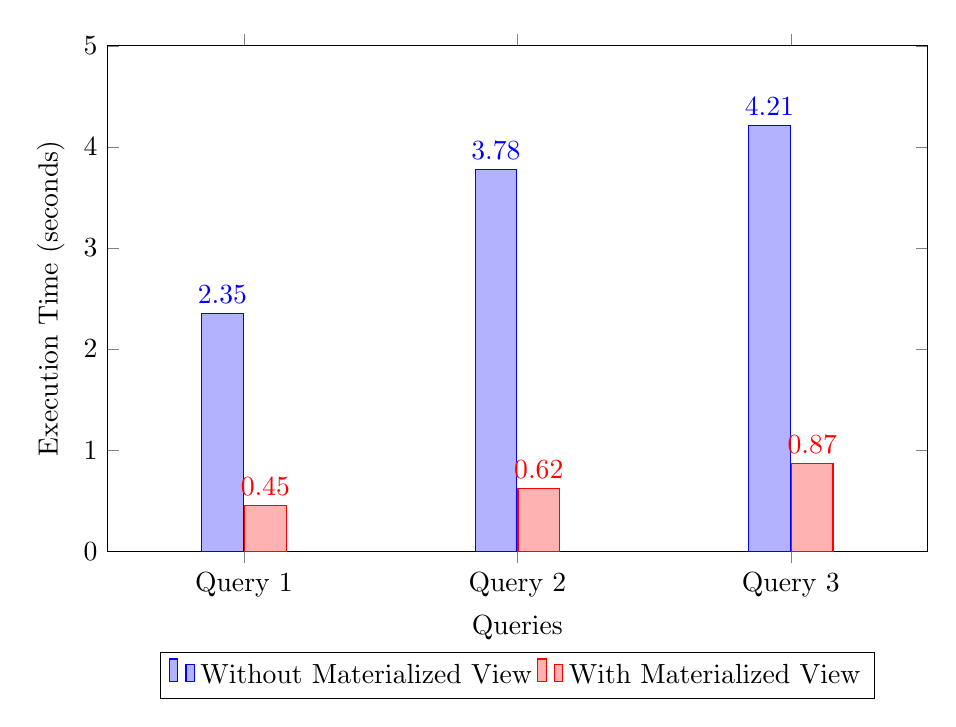
\begin{tikzpicture}
    \begin{axis}[
        width=12cm, height=8cm,
        ybar=0.5pt, % Bar style
        bar width=15pt,
        symbolic x coords={Query 1, Query 2, Query 3},
        xtick=data,
        ymin=0, ymax=5,
        ylabel={Execution Time (seconds)},
        xlabel={Queries},
        legend style={at={(0.5,-0.2)}, anchor=north, legend columns=-1},
        nodes near coords, % Show data labels
        enlarge x limits=0.25
    ]
        % Without Materialized View Data
        \addplot coordinates {(Query 1,2.35) (Query 2,3.78) (Query 3,4.21)};
        % With Materialized View Data
        \addplot coordinates {(Query 1,0.45) (Query 2,0.62) (Query 3,0.87)};
        
        \legend{Without Materialized View, With Materialized View}
    \end{axis}
\end{tikzpicture}

\begin{table}[h!]
    \centering
    \begin{tabular}{@{}lccc@{}}
        \toprule
        \textbf{Query} & \textbf{Without MV (s)} & \textbf{With MV (s)} & \textbf{Difference (\%)} \\ \midrule
        Query 1        & 2.35                   & 0.45                 & 80.85                   \\
        Query 2        & 3.78                   & 0.62                 & 83.61                   \\
        Query 3        & 4.21                   & 0.87                 & 79.34                   \\ \bottomrule
    \end{tabular}
    \caption{Execution Time Difference Between Queries With and Without Materialized Views}
    \label{tab:performance}
\end{table}


\begin{table}[h!]
    \centering
    \begin{tabular}{@{}lccc@{}}
        \toprule
        \textbf{Query} & \textbf{Without MV (s)} & \textbf{With MV (s)} & \textbf{Difference (\%)} \\ \midrule
        Query 1        & 2.35                   & 0.45                 & 80.85                   \\
        Query 2        & 3.78                   & 0.62                 & 83.61                   \\
        Query 3        & 4.21                   & 0.87                 & 79.34                   \\ \bottomrule
    \end{tabular}
    \caption{Performance Comparison for Queries With and Without Materialized Views}
    \label{tab:performance}
\end{table}

For example, the percentage difference for Query 1 is calculated as:
\[
\text{Difference (\%)} = \frac{\text{Without MV} - \text{With MV}}{\text{Without MV}} \times 100 = \frac{2.35 - 0.45}{2.35} \times 100 \approx 80.85\%
\]